% sage_latex_guidelines.tex V1.01, 11 June 2015

%\documentclass[Afour,sagev,times]{sagej}
\documentclass[Crown,sagev,times,doublespace]{sagej}


\usepackage{moreverb,url,color}
\usepackage[colorlinks,bookmarksopen,bookmarksnumbered,citecolor=red,urlcolor=red]{hyperref}

\newcommand\BibTeX{{\rmfamily B\kern-.05em \textsc{i\kern-.025em b}\kern-.08em
T\kern-.1667em\lower.7ex\hbox{E}\kern-.125emX}}

\def\volumeyear{2016}

\begin{document}

%\runninghead{Garc\'ia-S\'anchez et al.}
\runninghead{anonymous}
\title{Parallel Multi-objective optimization using co-evolutionary islands and search space overlapping}

%\author{Pablo Garc\'ia-S\'anchez, Julio Ortega, Jes\'us Gonz\'alez, \\Pedro Angel Castillo and Juan Juli\'an Merelo\affilnum{1}}
\author{ANONYMOUS FOR BLIND REVIEW \affilnum{1}}
\affiliation{\affilnum{1} ANONYMOUS FOR BLIND REVIEW}
\affiliation{\affilnum{1}Dept. of Computer Architecture and Computer Technology, University of Granada, Spain}

%\corrauth{Pablo Garc\'ia-S\'anchez,
%ETS. Ingenier\'ias en Inform\'atica y Telecomunicaci\'on and CITIC-UGR,
%C/Periodista Daniel Saucedo s/n,
%Universidad de Granada,
%18071, Granada, Spain.}

%\corrauth{ANONYMOUS FOR BLIND REVIEW.}

%\email{pablogarcia@ugr.es}
\email{anonymous}


\begin{abstract}
Multi-objective optimization methods have gained interest in the last years because the performance they can achieve solving real-world problems. Many of these problems usually require a high-dimensional decision space, and multi-objective Evolutionary Algorithms have been successfully used in the past. Due to the large computational cost these algorithms require, different parallelization and distribution methods have been proposed, with different parallel and distributed computer architectures to cope with them. One of the most extended methods are the distributed co-evolutionary evolutionary algorithms, where each processor only deals with a part of the decision space, that is, the individuals belonging to the same sub-population (island) explore the same subset of decision variables.  

In this paper, a new method to automatically adapt the overlapping sections of the individuals have been compared to other collaborative evolutionary methods.
Different number of islands, chromosome sizes and problems have been used. The analysis of the obtained experimental results, by using different 
metrics, shows that coevolutionary approaches can provide statistically significant improvements with respect to the base algorithm, being the method to automatically adapt the overlapping size the one to obtain the best performance during the same execution time. Results also show that the relation of the number of 
islands (subpopulations) to the length of the chromosome (number of decision variables) is also a relevant factor to determine the most efficient alternative to distribute the decision variables.
\end{abstract}









\keywords{Multi-objective algorithms, NSGA-II, Island model, distributed evolutionary algorithms, coevolution}

\maketitle

\section{Introduction}

Different approaches have been used to parallelize Evolutionary Algorithms (EAs), as each individual can be considered as an independent unit \citep{Alba13parallel}. Classic methods, such as the global parallel EAs (Master-Slave), or the spatially structured algorithms (Island model or Cellular EAs) have been applied successfully in the past \citep{Folino03cellular,Alba02Parallelism}.  In the case of Multi-Objective Evolutionary Algorithms (MOEAs), these approaches \citep{Luna15Survey} need to deal with a whole solution set called Pareto Front (PFs). This imply to use different distribution and sharing mechanisms, as there exist a tension between the speedup achievable from parallelization and the need to globally recombine the results to accurately identify the PF \citep{Branke04Parallelizingcone}.


The application of MOEAs to solve real-world problems have gained attention in the last years \citep{Luna15Survey,Mukhopadhyay14Survey,Chavez15MO,Hidalgo16residualstress}. These kind of problems requires a high number of variables, meaning that the EAs need to deal with large individuals and spent significant extra time for crossover, mutation and migration. Different authors have proposed methods to divide the decision space (the chromosome) to improve the performance and solution quality. In this aspect, the co-evolution model is a dimension-distributed model where a high-dimensional problem is divided into lower dimensional problems \citep{Gong15models,Tonda12cooperative}, and evolved separately. One example of application of this technique was described in \citep{Kimovski15Parallel}. The method presented in that works involves different workers that evolve sub-populations created and recombined by a master process, which performs different recombination alternatives from the parts returned by worker processes. A high dimensional problem was used to compare these
alternatives. In \citep{Dorronsoro13superlinear}, a distributed coevolutionary island model was used.  Although in both previous works significant speedups were attained, only a low number of nodes were used (8). However, when increasing the number of islands, the division of each section of the chromosome becomes smaller, and the scalability may be affected by obtaining lower quality solutions in the same amount of time.

In our preliminary work in \citep{Garcia16hpmoonANONYMOUS} we tried to demonstrate that using overlapped sections of the chromosome in a coevolutionary multi-objective island-based algorithm can improve the quality of the solutions in the same computing time when the number of islands increases. We discovered that the most adequate overlapping size may vary depending on a relation between the number of islands and the individual size. Moreover, the experiments were conducted in a mono-processor and synchronous island model. This motivates us to continue this research line, but this time, proposing a new method to automatically adapt the size of the overlapped sections, but also, performing all the experiments in a real cluster with up to 128 nodes, with extra number of islands.


The hypothesis of this paper is that using overlapped sections of the chromosome, calculated depending the number of islands to use, in a coevolutionary multi-objective island-based algorithm can improve the quality of the solutions in the same computing time with respect to the baseline, disjoint and partly overlapped methods. To demonstrate this, a new overlapping islands scheme has been compared with a baseline version of a distributed NSGA-II \citep{Deb00NSGAII}, a coevolutionary disjoint section approach, and a fixed-size overlapped method. Different benchmarks problems and different large number of islands have been used. Results show that this new technique can improve different quality indicators in the same amount of time when the problem size is large. 

The rest of the paper is organized as follows: after a background in parallelization in MOEAs, 
the compared algorithms and the used methodology are presented. %PABLO: no puedo usar \ref{sec:met} porque la plantilla de esta revista no lo coge :/ (y además no tienen número)
Then, the results of the experiments are shown, followed by conclusions and suggestions for future work lines.


%%%%%%%%%%%%%%%%%%%%%%%%%%%%%%  STATE OF THE ART  %%%%%%%%%%%%%%%%%%%%%%%%%%%%%
%
\section{State of the Art}
\label{sec:soa}

Evolutionary algorithms (EAs) \citep{DBLP:series/ncs/EibenS15,DeJong2006} are bio-inspired meta-heuristics that can be effectively used to find nearly optimal solutions for optimization problems. Usually an EA starts by generating a set of random solutions, called \emph{population}, following a user-defined description. Then, it evaluates each candidate solution, called \emph{individual}, assigning it a \emph{fitness} value, that describes how good the individual is, with regards to the target problem. New solutions are then generated by the application of \emph{operators} that either mutate a single solution or recombine different existing solutions. After each iteration, called \emph{generation}, the least fit individuals are removed, and the process continues until a user-defined stop condition is met.

Multi-objective optimization problems (MOP) are those where several objectives have to be simultaneously optimized \citep{Mora13paretobased}. Solving a MOP implies maximize or minimize a function composed of several cost functions (one per objective). In these problems the aim is to obtain a set of solutions that are better than the rest, considering all the objectives; this set is known as the Pareto Front. The solutions in this set are {\em non-dominated}, that is, none is better than the others for all the objectives. MOEAs are sub-set of EAs used to solve MOPs. One of the most well-known and referenced MOEAs \citep{Dorronsoro13superlinear} is the {\em Non-dominated Sorting Genetic Algorithm} (NSGA-II) \citep{Deb00NSGAII}. Classical genetic operators are applied to all the individuals, and divided into different ranks (based on the dominance) to be selected for the next generations.


Since the early 2000s, the distributed and parallel Evolutionary Algorithms have been used, mostly to take the most from systems such as clusters or grids \citep{Talbi08Parallel}. But in the case of MOEAs, the distribution and parallelization is not as direct as in single-objective EAs. This is because in different steps of the algorithm a whole set of dependent solutions, the Pareto Front, should be managed as a whole, spending time in gathering all individuals from the different processors or islands.

To solve this issue, some authors have proposed the usage of Master-Slave approaches. For example,  \citep{Durillo08masterslave} compared different master-slave approaches: synchronous generational, asynchronous generational and asynchronous steady-state, being the latter the most promising option. The method proposed by Hiroyasu \citep{Hiroyasu07discussion} generates offspring depending on the computational power.

The work by Deb et al. \citep{Deb03distributed} was one of the first approaches for distributed MOEAs (dMOEAs). In that work, the dominance of solutions was divided into the islands using a transformation of coordinates. Their authors concluded that dividing the search space is a good idea, but achieve this is not trivial. Other approaches for dividing the search space include objective separation in different processors \citep{Xiao03specialized}, or divide in two populations: one for elite and other search \citep{Wang09parallel}. Martens, in \citep{Martens13asynchronous} generated a Barabasi-Albert network as the island topology, and selection based on migrating individuals from a not-crowded area and acceptance based on diversity. 


More similar approaches to the one presented here were studied in the
next two works, also using cooperative coevolution for high-dimensional problems. 
Dorronsoro et al. \citep{Dorronsoro13superlinear} obtained super-linear performance
in several instances using cooperative coevolution, focusing each island on a portion of the chromosome. However, in some instances the parallel version 
improved the sequential version. Kimovski et al. \citep{Kimovski15Parallel} proposed a
master-slave method that splits the population into several processors,
each one running in parallel a MOEA that only affects some portion of
the individuals. After a certain number of generations, the master
process receives all the sub-populations to be combined. Different
combination alternatives in this step are compared. Up to 8 processors
were used in the experimental setup. Our approach in this paper does not
broadcast all solutions to all islands for recombination, as previous
works, but only one solution to a random island, needing less
communication time. Besides, the maximum number of islands of
Dorronsoro or Kimovsky approaches was 8, while in this paper we have
used up to 128 islands. 

Lately, some researchers \citep{cheng2015adaptive} have focused on
working on solution space, dividing the Pareto front in different
clusters in order to model it. This {\em divide and conquer} approach
is readily paralellizable and, in the sense of giving the
responsibility of different parts of the search space to different
modules, is similar to the one presented in this paper.

In our previous work \citep{Garcia16hpmoonANONYMOUS} we used some of the previous ideas to compare two co-evolutionary dMOEAs. The first one divided the chromosome in $P$ sections, being $P$ the number of islands. Every island $p$ only performed the mutation and crossover in that part ($p_{th}$) of the chromosome, while the fitness was calculated using the whole individual. After a certain number of generations, individuals were migrated randomly to other islands. The performance metrics were calculated at the end of the run. The second method, coevolution with overlapping islands, used the $p_{th-1}$ and $p_{th+1}$ sections of each chromosome, besides the $p_{th}$ part. During the same amount of time both methods obtained better results than a baseline algorithm that dealt with the whole chromosome in each island for crossover and mutation. We discovered that the performance using one or another method depends on the number of sections of the individuals and the number of islands used. This motivates us to find a new adaptive method to select this number of sections of the chromosome to use, depending on the number of islands. Moreover, previous experiments were performed on a single processor synchronous island model with a limited number of islands (8, 32 and 128). In this paper,  8, 16, 32, 64 and 128 islands have been used, and this time, the experiments have been run on a real cluster. Therefore, at the same time we are proposing an adaptive method to divide the individual search space, we are validating the previous methods.


We will describe how we have tested our approach in the next Section.




%
%%%%%%%%%%%%%%%%%%%%%%%%%%%%%%  METHODOLOGY  %%%%%%%%%%%%%%%%%%%%%%%%%%%%%
%

\section{Coevolutionary algorithms compared}
\label{sec:coevo}

In this paper we analyse several coevolutionary algorithms we have implemented by using a parallel multi-objective baseline algorithm (B) as a framework. Here, we have used the NSGA-II algorithm as the baseline algorithm. The population is distributed among $P$ islands. After a fixed number of generations, one individual in a given island is migrated to another random island, thus avoiding to synchronize the global Pareto Front (PF) every certain number of generations as other methods described in Section 2 do. At the end of the run, the Pareto Fronts of all islands are aggregated into a new one, and the quality measures are evaluated.
Different coevolutionary alternatives can be devised to evolve the subpopulations according to the decision space to be explored by each islands. Here we will consider three methods in which each island only performs crossover and mutation in specific sections of the individuals.



%This algorithm is a regular NSGA-II algorithm distributed along a number $P$ of islands. After a fixed number of generations, one individual is migrated to another random island. At the end of the run, PFs of all islands are aggregated in a new one in order to compute the quality measures. This baseline method has been chosen as it does not require synchronization of the global PF every certain number of generations, as other methods described in Section 2 do.
%% some justification on why this was chosen - JJ PABLO: Added 
%
%% And some liaison to next subsection - JJ
%This method will be compared to different coevolutionary approaches that are similar to the baseline, with the exception on the decision space to explore in each island.
%Three different coevolutionary methods have been used. In all these methods, each island only performs crossover and mutation in specific sections of the individuals.

As in the baseline, every certain number of generations, an individual is migrated to another random island.  In the new island, this individual will be considered as one of the others in the island, crossed and mutated in the same way, depending on the island identifier. Note that, on the contrary of other works such as the ones described by Talbi et al. \citep{Talbi08Parallel} all the islands deal with complete chromosomes for fitness calculation, so our approach can deal with no decomposable problems. The proposed methods  are as follows:

\subsection{Coevolution with disjoint islands (D)} 
In this approach, each individual of size $L$ is split into $P$ chunks of size $L/P$. Every island $p$ only performs crossover and mutation on the $p_{th}$ part of the individuals. Figure \ref{fig:disjoint} describes this approach.  

\begin{figure*}
\centering
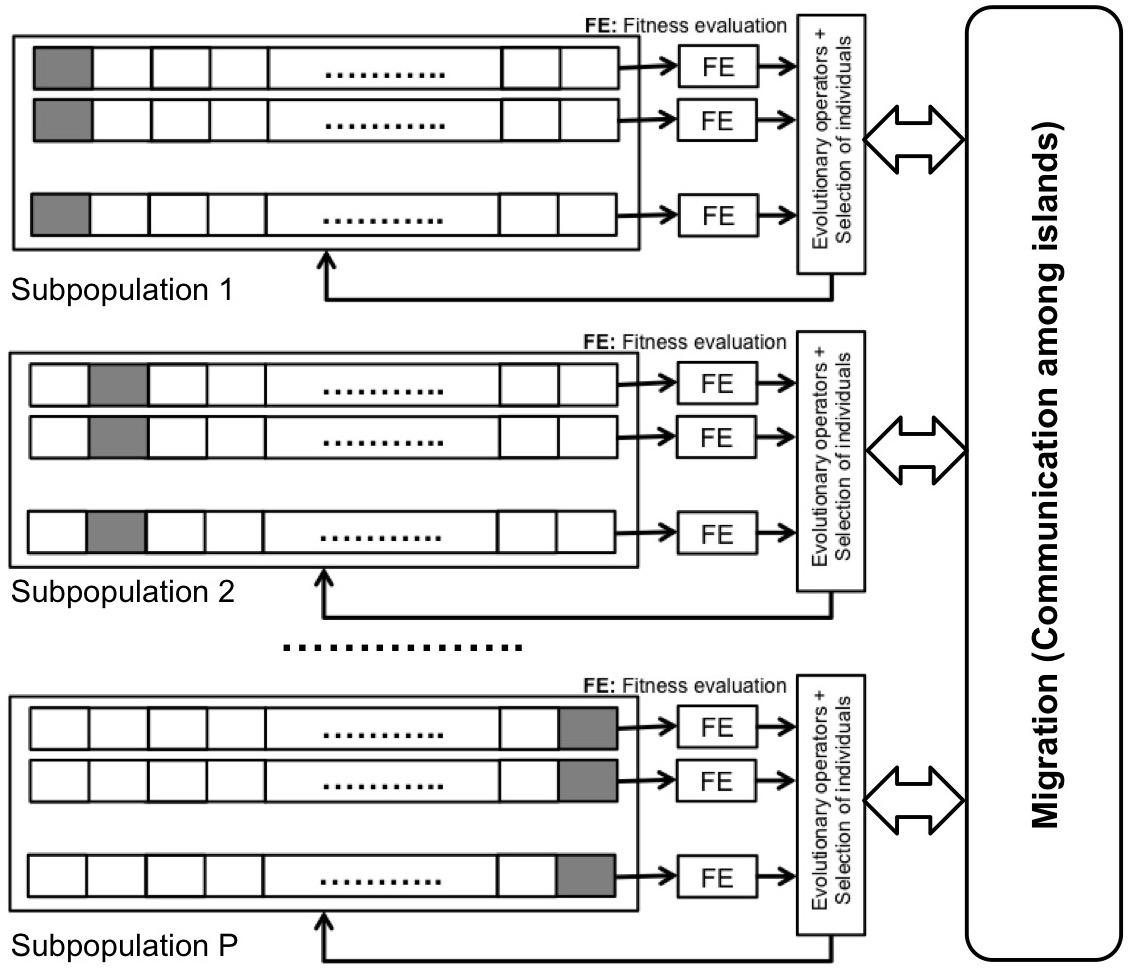
\includegraphics[width=12cm]{islandDisjoint.jpg}
\caption{Disjoint algorithm: every island $p$ only modifies the $p_{th}$ components (in grey) of the individuals.}
\label{fig:disjoint}
\end{figure*}

\subsection{Coevolution with overlapping islands (O)}
This approach is similar to the previous one, but every island also uses the $p+1$ and $p-1$ (module size) chunks of the individual for crossover and migration. Therefore, some kind of overlapping of the crossed and mutated parts exists between islands. Figure \ref{fig:overlapping} shows the affected parts of the individuals in
each island. 

\begin{figure*}
\centering
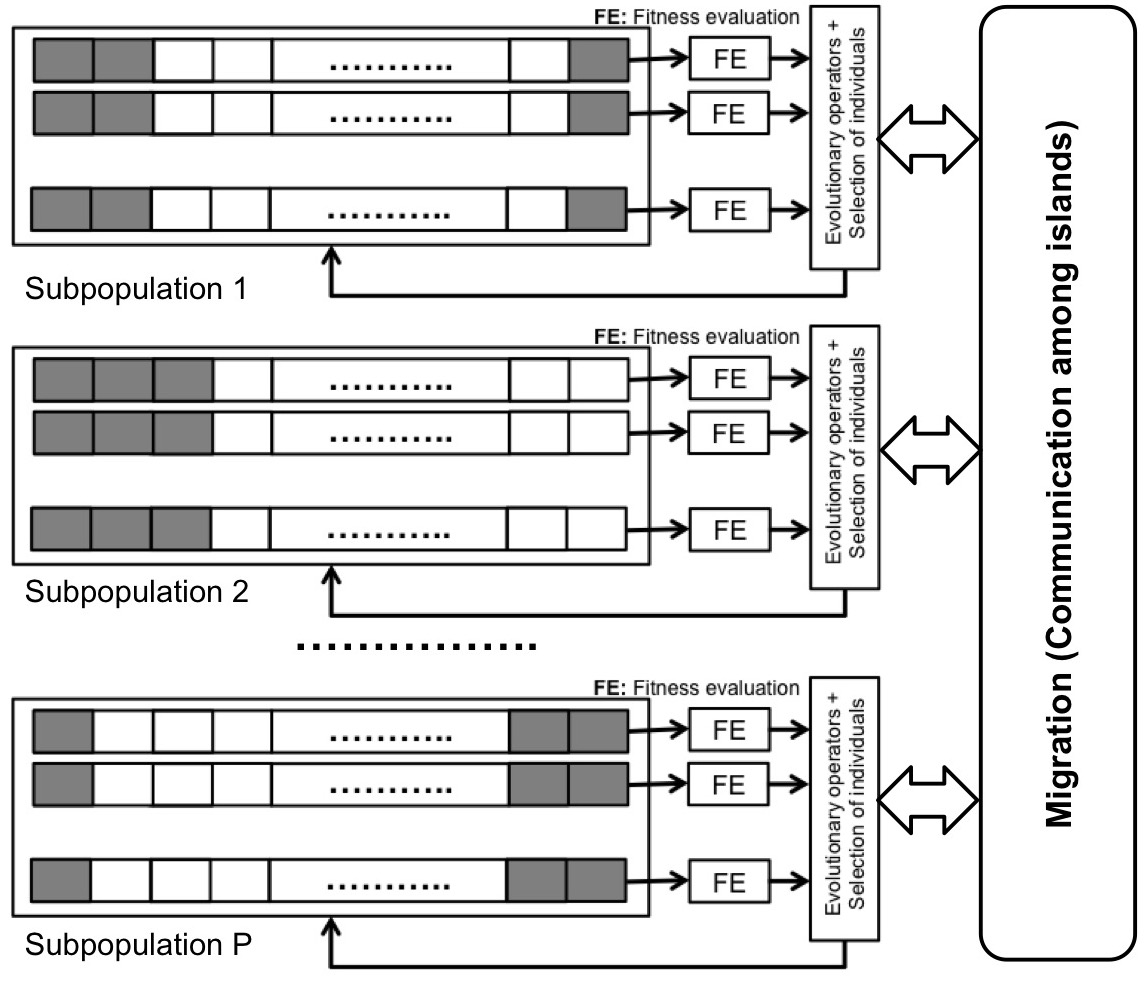
\includegraphics[width=12cm]{islandNoDisjoint.jpg}
\caption{Overlapping algorithm: every island $p$ modifies the  $p+1$,
  $p_{th}$ and $p-1$  components (in grey) of the individuals.}
  \label{fig:overlapping}
\end{figure*}

\subsection{Adaptive coevolution with overlapping islands (A)} 
As in the previous method, the sections to address are overlapped, but instead using one extra section on each side of the $p$ section ($p+1$ and $p-1$), it uses $c$ fragments on each side ($p+c$ and $p-c$), being $c$ a value depending on the number of islands. As a first approach to automatically calculate this value the results shown in \citep{Garcia16hpmoonANONYMOUS} have been used as a base to obtain $c$. In that work, the overlapped method ($c=1$) obtained better results when the number of islands were $>$8. So, we have used the formula $c=round(0.2*P-1)/2$ to calculate the extra sections to overlap. Therefore, when $P=8$ then $c=0$ (equivalent to D), when $P=16$ then $c=1$ (equivalent to O), and so on. Figure \ref{fig:adaptive} explains this method.

\begin{figure*}
\centering
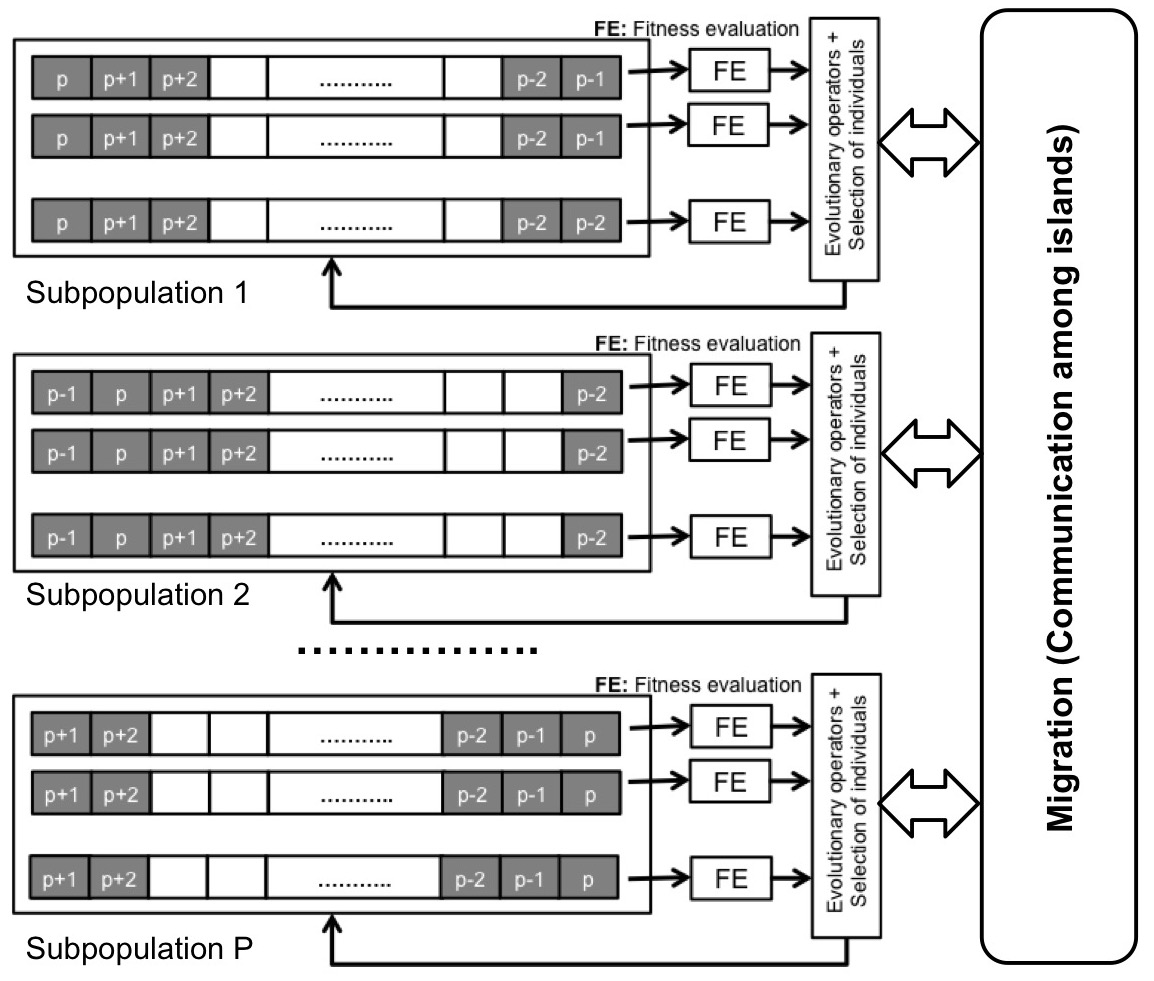
\includegraphics[width=12cm]{islandAdaptive.jpg}
\caption{Adaptive overlapping algorithm: every island $p$ modifies the  $p+c$,
  $p_{th}$ and $p-c$  components (in grey) of the individuals. $c$ is calculated depending on the number of islands. In this case, $c=2$.}
  \label{fig:adaptive}
\end{figure*}
% --------------------------------------------------------------


%%%%%%%%%%%%%%%%%%%%%%%%%%  EXPERIMENTS AND RESULTS  %%%%%%%%%%%%%%%%%%%%%%%%%%
%
\section{Experiments and Results}
\label{sec:res}

This section describes the quality indicators used and the experimental setup. The chosen quality indicators, are:

\begin{itemize}
\item Hypervolume (HV): measures the area formed by all non-dominated solutions found with, respect to a reference point. Higher values imply better quality of the PF. Figure \ref{fig:hypervolume} clarifies how the hypervolume is calculated.
\item Inverted Generational distance (IGD): calculates the distance of the obtained set of solutions to the optimal PF. Therefore, this metric requires the optimal PF found in the literature, or the theoretical one. In this metric, the lower the better. %Pablo: theoretical?
\item Spread (S): Measures the spread between solutions, taking into account the euclidean distance between consecutive solutions. As in previous metric, the lower value, the better, as it implies solutions distributed along all the PF.
\end{itemize}

\begin{figure}
\centering
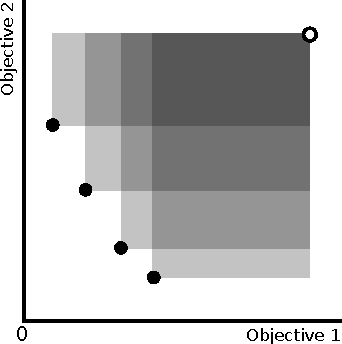
\includegraphics[width=6cm]{hypervolume.pdf}
\caption{Hypervolume calculation. Areas from Pareto Front solutions (black points) to a reference point (white point) are added.}
\label{fig:hypervolume}
\end{figure}


These metrics have been used extensively, especially in some of the papers presented in Section 2.

The previously described four approaches have been run with two different chromosome lengths ($L$): 512 and 2048. Different number of islands ($P$) have also been compared: 8, 16, 32, 64 and 128. This maximum number of islands have also been  used in previous work in the literature \citep{Martens13asynchronous}. The crossover and mutation chosen, SBX and polynomial, have also been  used previously by other authors in \citep{Durillo08masterslave}. 

ZDT \citep{zdt2000a} has been chosen as a benchmark, since it is the most widely used in this area \citep{Deb03distributed,Martens13asynchronous,Wang09parallel,Durillo08masterslave}. The optimal PF distribution used for comparison has 1000 solutions \footnote{Optimal PFs are available at:   \url{http://www.tik.ee.ethz.ch/sop/download/supplementary/testproblems/}.}. 





Termination criterion used has been the running time: 25 seconds for dimension 512 and 100 (four times more) for 2048. We have used the time instead the number of evaluations firstly because our hypothesis argue that the time saved in crossover and mutation can be spent on improving the sub-populations and more operations and migrations can be achieved. Also, we are using different number of islands (with different sub-population sizes) that could lead to different execution times, so it would be difficult to compare different times and quality solutions at the same time.

\begin{table*}
\begin{center}
\begin{tabular}{|c|c|}
\hline
{\em Parameter Name} & {\em Value} \\ \hline
Number of islands ($P$) & 8, 16, 32, 64 and 128 \\ \hline
Chromosome size ($L$) & 512 and 2048 \\ \hline
Execution time (s) & 25 (for 512) and 100 (for 2048) \\ \hline \hline
Global population size ($N$) & 1024 \\ \hline
Selection type & Binary Tournament Selection \\ \hline
Replacement type & Generational \\ \hline 
Crossover type & SBX \\ \hline
Mutation  type & Polynomial\\ \hline
Mutation probability & 1/$L$ \\ \hline
Generations between migration & 5 \\ \hline
Individuals per migration & 1 \\ \hline
Selection for migration & Binary Tournament\\ \hline
Runs per configuration & 30 \\ \hline
\end{tabular}
\caption{Parameters and operators used in the experiments.}
\label{tab:parameters}
\end{center}
\end{table*}

The ECJ framework \citep{ECJ} has been used to run the
experiments. Specific operators have been developed as new modules for
ECJ, and they can be downloaded from our GitHub repository under a
LGPL V3 License
%\footnote{\url{https://github.com/hpmoon/hpmoon-islands}}. 
\footnote{\url{https://ANONYMOUS-REPOSITORY}}. 
The
island model has been executed synchronously, using the ECJ Internal
Island Model, in a CentOS 5.4 machine with Intel(R) Xeon(R) CPU E5520
@2.27GHz, 16 GB RAM, with Java Version 1.6.0\_16.


Different metrics, explained in the previous section, have been used to calculate the quality of the obtained PFs in each configuration. As some of the metrics  (such as HV) require a reference point to be calculated, the point (1,9) has been chosen as reference, as none of the generated PFs in all runs are dominated by it. Metrics are then normalized with respect to that point. A Kruskall-Wallis significance test has been performed to the metrics of all runs of the configurations, as the Kolmogorov-Smirnov test detected non-normal distributions. The average results for each configuration are shown in Table \ref{tab:results512} (for 512 dimensions) and \ref{tab:results2048} (for 2048). As previously explained, when $P=8$ the results of A are equivalent to the obtained with D (because $c=0$), and when $P=16$ they are equivalent to O ($c=1$).


\begin{table*}
\centering
\resizebox{14cm}{!}{
\begin{tabular}{|c||c|c|c|c||c|c|c|c||c|c|c|c||}
\hline
	&	\multicolumn{4}{|c|}{HV}													&	\multicolumn{4}{|c|}{Spread}														&	\multicolumn{4}{|c|}{IGD}														\\ \hline
%\multicolumn{13}{|c|}{2048 dimenOionO}																																													\\ \hline
\#Island	&	B		&	D		&	O			&	A			&	B		&	D			&	O			&	A			&	B		&	D		&	O		&	A					\\ \hline
\multicolumn{13}{|c|}{ZDT1}																																													\\ \hline
8	&	0.900		&	0.816		& \textbf{	0.926	}		&	Equiv. D			& \textbf{	0.729	}	&	1.041			&	0.898			&	Equiv. D			&	0.013		&	0.029		& \textbf{	0.007	}	&	Equiv. D					\\
16	& \textbf{	0.880	}	&	0.675		&	0.839			&	Equiv. O			& \textbf{	0.721	}	&	0.897			&	0.983		D	&	Equiv. O			& \textbf{	0.017	}	&	0.062		&	0.025		&	Equiv. O					\\
32	& \textbf{	0.829	}	&	0.618		&	0.698			&	0.790			& \textbf{	0.763	}	&	0.879			&	0.886		D	&	0.913	DO		& \textbf{	0.027	}	&	0.076		&	0.056		&	0.036					\\
64	& \textbf{	0.769	}	&	0.596		&	0.628			&	0.736			& \textbf{	0.820	}	&	0.897			&	0.872			&	0.890	DO		& \textbf{	0.040	}	&	0.080		&	0.071		&	0.047					\\
128	& \textbf{	0.707	}	&	0.585		&	0.598			&	0.668			& \textbf{	0.850	}	&	0.956			&	0.883			&	0.910	O		& \textbf{	0.053	}	&	0.083		&	0.079		&	0.062					\\ \hline
\multicolumn{13}{|c|}{ZDT2}																																													\\ \hline
8	&	0.830		&	0.786		& \textbf{	0.851	}		&	Equiv. D			& \textbf{	0.866	}	&	0.996			&	0.987		D	&	Equiv. D			&	0.023		&	0.037		& \textbf{	0.017	}	&	Equiv. D					\\
16	& \textbf{	0.810	}	&	0.601		&	0.776			&	Equiv. O			& \textbf{	0.916	}	&	0.990			&	1.005		D	&	Equiv. O			& \textbf{	0.029	}	&	0.091		&	0.040		&	Equiv. O					\\
32	& \textbf{	0.756	}	&	0.498		&	0.617			&	0.682			& \textbf{	0.976	}	& \textbf{	0.976	}	B	& \textbf{	0.978	}	BD	&	1.054			& \textbf{	0.045	}	&	0.119		&	0.086		&	0.068					\\
64	& \textbf{	0.668	}	&	0.451		&	0.504			&	0.601			&	1.002		& \textbf{	0.976	}		& \textbf{	0.974	}	D	&	1.025	B		& \textbf{	0.070	}	&	0.132		&	0.117		&	0.091					\\
128	& \textbf{	0.576	}	&	0.434		&	0.452			&	0.526			&	1.002		&	1.023			& \textbf{	0.978	}		&	1.015	BD		& \textbf{	0.096	}	&	0.137		&	0.132		&	0.110					\\ \hline
\multicolumn{13}{|c|}{ZDT3}																																													\\ \hline
8	&	0.928		&	0.838		& \textbf{	0.951	}		&	Equiv. D			& \textbf{	0.869	}	&	1.028			&	0.983		D	&	Equiv. D			& \textbf{	0.008	}	&	0.018		&	0.005		&	Equiv. D					\\
16	& \textbf{	0.903	}	&	0.715		&	0.870			&	Equiv. O			& \textbf{	0.846	}	&	0.899			&	0.960			&	Equiv. O			& \textbf{	0.011	}	&	0.032		&	0.014		&	Equiv. O					\\
32	& \textbf{	0.857	}	&	0.655		&	0.737			&	0.824			& \textbf{	0.845	}	&	0.879			&	0.873		D	&	0.881	DO		& \textbf{	0.016	}	&	0.039		&	0.030		&	0.019					\\
64	& \textbf{	0.796	}	&	0.632		&	0.662			&	0.761			& \textbf{	0.859	}	&	0.887			&	0.885		D	&	0.879	BDO		& \textbf{	0.023	}	&	0.042		&	0.038		&	0.027					\\
128	& \textbf{	0.738	}	&	0.620		&	0.633			&	0.705			& \textbf{	0.882	}	&	0.968			& \textbf{	0.888	}	B	&	0.911			& \textbf{	0.029	}	&	0.044		&	0.042		&	0.033					\\ \hline
\multicolumn{13}{|c|}{ZDT6}																																													\\ \hline
8	&	0.268		&	0.223		& \textbf{	0.298	}		&	Equiv. D			& \textbf{	0.988	}	& \textbf{	0.972	}	B	& \textbf{	0.996	}	B	&	Equiv. D			& \textbf{	0.173	}	&	0.191		&	0.160		&	Equiv. D					\\
16	& \textbf{	0.243	}	&	0.113		&	0.219			&	Equiv. O			& \textbf{	0.995	}	& \textbf{	0.987	}	B	& \textbf{	0.987	}	BD	&	Equiv. O			& \textbf{	0.184	}	&	0.240		&	0.193		&	Equiv. O					\\
32	& \textbf{	0.196	}	&	0.071		&	0.115			&	0.162			& \textbf{	0.998	}	& \textbf{	0.989	}	B	& \textbf{	0.988	}	BD	&	1.005	B		& \textbf{	0.204	}	&	0.257		&	0.238		&	0.220					\\
64	& \textbf{	0.145	}	&	0.056		&	0.075			&	0.120			&	0.996		&	0.986		B	& \textbf{	0.983	}	D	&	0.998	B		& \textbf{	0.226	}	&	0.264		&	0.255		&	0.235					\\
128	& \textbf{	0.104	}	&	0.049		&	0.055			&	0.084			&	0.993		&	1.007			& \textbf{	0.979	}		&	0.998	BD		& \textbf{	0.244	}	&	0.266		&	0.263		&	0.251					\\ \hline

\end{tabular}
}
\caption{Average quality metrics obtained after 30 runs per configuration, for the 4 methods compared: baseline (B), disjoint (D), overlapped (O) and adaptive overlapped (A), using a chromosome length of 512 dimensions. Acronyms next to values indicate that there is not significant difference with respect to that method for that value. Best values are marked in bold.}
\label{tab:results512}
\end{table*}



\begin{table*}
\centering
\resizebox{13cm}{!}{
\begin{tabular}{|c||c|c|c|c||c|c|c|c||c|c|c|c||}
\hline
	&	\multicolumn{4}{|c|}{HV}													&	\multicolumn{4}{|c|}{Spread}														&	\multicolumn{4}{|c|}{IGD}														\\ \hline

\#Island	&	B		&	D		&	O			&	A			&	B		&	D			&	O			&	A			&	B		&	D		&	O		&	A					\\ \hline
\multicolumn{13}{|c|}{ZDT1}																																													\\ \hline
8	&	0.891		& \textbf{	0.953	}	&	0.937			&	Equiv. D			& \textbf{	0.681	}	& \textbf{	0.635	}	B	&	0.661		D	&	Equiv. D			&	0.015		& \textbf{	0.002	}	&	0.005		&	Equiv. D					\\
16	&	0.884		&	0.850		& \textbf{	0.942	}		&	Equiv. O			& \textbf{	0.705	}	&	0.908			& \textbf{	0.670	}	B	&	Equiv. O			&	0.016		&	0.022		& \textbf{	0.004	}	&	Equiv. O					\\
32	&	0.851		&	0.674		&	0.859		B	& \textbf{	0.900	}		& \textbf{	0.754	}	&	0.868			&	0.826		D	& \textbf{	0.763	}	B	&	0.023		&	0.062		&	0.020	B	& \textbf{	0.012	}				\\
64	& \textbf{	0.800	}	&	0.608		&	0.697			& \textbf{	0.824	}	B	& \textbf{	0.808	}	&	0.880			& \textbf{	0.861	}	B	& \textbf{	0.823	}	B	&	0.033		&	0.078		&	0.056		& \textbf{	0.027	}				\\
128	&	0.735		&	0.582		&	0.613			& \textbf{	0.745	}		& \textbf{	0.841	}	&	0.888			&	0.878		D	&	0.865		O	&	0.047		&	0.084		&	0.075		& \textbf{	0.043	}				\\ \hline
\multicolumn{13}{|c|}{ZDT2}																																													\\ \hline
8	&	0.832		& \textbf{	0.895	}	&	0.869			&	Equiv. D			& \textbf{	0.849	}	& \textbf{	0.886	}	B	&	0.853		D	&	Equiv. D			&	0.023		& \textbf{	0.006	}	&	0.013		&	Equiv. D					\\
16	&	0.831		&	0.833	B	& \textbf{	0.884	}		&	Equiv. O			& \textbf{	0.810	}	&	1.001			& \textbf{	0.802	}	B	&	Equiv. O			&	0.023		&	0.022	B	& \textbf{	0.009	}	&	Equiv. O					\\
32	&	0.800		&	0.628		&	0.800		B	& \textbf{	0.817	}		& \textbf{	0.848	}	&	0.974			&	0.983		D	&	0.908			&	0.031		&	0.082		&	0.032	B	& \textbf{	0.027	}				\\
64	& \textbf{	0.729	}	&	0.491		&	0.623			&	0.716			& \textbf{	0.909	}	&	0.967			&	0.979		D	& \textbf{	0.997	}	BD	& \textbf{	0.052	}	&	0.121		&	0.084		& \textbf{	0.055	}	B			\\
128	& \textbf{	0.630	}	&	0.441		&	0.500			& \textbf{	0.614	}	B	& \textbf{	0.957	}	&	0.989			&	0.978		D	& \textbf{	0.994	}	BO	& \textbf{	0.080	}	&	0.136		&	0.119		& \textbf{	0.085	}	B			\\ \hline
\multicolumn{13}{|c|}{ZDT3}																																													\\ \hline
8	&	0.917		& \textbf{	0.971	}	&	0.960			&	Equiv. D			& \textbf{	0.843	}	& \textbf{	0.854	}	B	&	0.868		D	&	Equiv. D			&	0.009		& \textbf{	0.001	}	&	0.004		&	Equiv. D					\\
16	&	0.911		&	0.876	B	& \textbf{	0.963	}		&	Equiv. O			& \textbf{	0.864	}	&	0.899		B	& \textbf{	0.837	}	B	&	Equiv. O			&	0.010		&	0.014		& \textbf{	0.003	}	&	Equiv. O					\\
32	&	0.884		&	0.710		&	0.883		B	& \textbf{	0.931	}		& \textbf{	0.856	}	& \textbf{	0.870	}	B	& \textbf{	0.842	}	B	& \textbf{	0.842	}	BDO	&	0.013		&	0.032		&	0.013	B	& \textbf{	0.008	}				\\
64	&	0.828		&	0.645		&	0.728			& \textbf{	0.854	}		& \textbf{	0.878	}	& \textbf{	0.896	}	B	& \textbf{	0.871	}	BD	& \textbf{	0.873	}	BDO	& \textbf{	0.019	}	&	0.040		&	0.030		& \textbf{	0.016	}	B			\\
128	& \textbf{	0.770	}	&	0.620		&	0.651			& \textbf{	0.773	}	B	& \textbf{	0.887	}	& \textbf{	0.901	}	B	& \textbf{	0.890	}	BD	& \textbf{	0.885	}	BDO	& \textbf{	0.026	}	&	0.043		&	0.039		& \textbf{	0.025	}	B			\\ \hline
\multicolumn{13}{|c|}{ZDT6}																																													\\ \hline
8	&	0.271		& \textbf{	0.398	}	&	0.323			&	Equiv. D			& \textbf{	0.982	}	& \textbf{	0.982	}	B	&	0.994			&	Equiv. D			&	0.171		& \textbf{	0.115	}	&	0.149		&	Equiv. D					\\
16	&	0.275		&	0.295	B	& \textbf{	0.354	}		&	Equiv. O			& \textbf{	0.981	}	& \textbf{	0.970	}	B	&	1.006			&	Equiv. O			&	0.170		&	0.161	B	& \textbf{	0.136	}	&	Equiv. O					\\
32	&	0.239		&	0.123		&	0.240			& \textbf{	0.254	}		& \textbf{	0.989	}	& \textbf{	0.991	}	B	& \textbf{	0.982	}	BD	& \textbf{	0.999	}	BD	&	0.186		&	0.235		&	0.185	B	& \textbf{	0.179	}				\\
64	& \textbf{	0.184	}	&	0.068		&	0.125			& \textbf{	0.178	}	B	& \textbf{	0.985	}	& \textbf{	0.982	}	B	& \textbf{	0.992	}	B	& \textbf{	0.995	}	BO	& \textbf{	0.209	}	&	0.259		&	0.235		&	0.212					\\
128	& \textbf{	0.128	}	&	0.051		&	0.071			& \textbf{	0.124	}	B	& \textbf{	0.991	}	& \textbf{	0.992	}	B	& \textbf{	0.988	}	BD	&	1.003			& \textbf{	0.233	}	&	0.266		&	0.257		& \textbf{	0.235	}	B			\\ \hline

\end{tabular}
}
\caption{Average quality metrics obtained after 30 runs per configuration, for the 4 methods compared: baseline (B), disjoint (D), overlapped (O) and adaptive overlapped (A), using a chromosome length of 2048 dimensions. Acronyms next to values indicate that there is not significant difference with respect to that method for that value. Best values are marked in bold.}
\label{tab:results2048}
\end{table*}






\begin{table*}
\centering
\resizebox{12cm}{!}{
\begin{tabular}{|c||c|c|c|c||c|c|c|c||}
\hline
	&	\multicolumn{4}{|c|}{Average solutions per island}													&	\multicolumn{4}{|c|}{Generations}															\\ \hline

\#Island	&	B		&	D		&	O			&	A			&	B		&	D			&	O			&	A				\\ \hline
\multicolumn{9}{|c|}{ZDT1}																				\\ \hline
8	&	182.700		&	128.500		&	158.167			&	Equiv. D			&	397.367		&	776.967			&	603.667			&	Equiv. D				\\
16	&	132.567		&	43.633		&	76.167			&	Equiv. O			&	567.933		&	908.467			&	838.000			&	Equiv. O				\\
32	&	102.200		&	37.533		&	34.133	D		&	52.033			&	731.067		&	959.067			&	938.167			&	917.000				\\
64	&	81.100		&	46.267		&	26.300			&	30.167		O	&	846.733		&	978.733			&	972.567			&	927.133	B			\\
128	&	77.167		&	57.767		&	35.767			&	29.167		O	&	923.133		&	984.767			&	984.233	D		&	967.933				\\ \hline
\multicolumn{9}{|c|}{ZDT2}																															\\ \hline
8	&	122.700		&	91.633		&	108.833	BD		&	Equiv. D			&	398.167		&	772.000			&	605.100			&	Equiv. D				\\
16	&	94.867		&	28.033		&	62.467			&	Equiv. O			&	574.567		&	908.433			&	840.900			&	Equiv. O				\\
32	&	56.633		&	11.433		&	19.467	D		&	31.567			&	735.867		&	960.167			&	939.200			&	904.900				\\
64	&	33.467		&	10.267		&	9.367	D		&	19.067			&	849.900		&	978.600			&	972.167			&	929.800	B			\\
128	&	22.833		&	12.633		&	7.800			&	13.967		D	&	929.433		&	984.567			&	984.233	D		&	971.700				\\ \hline
\multicolumn{9}{|c|}{ZDT3}																															\\ \hline
8	&	212.900		&	129.233		&	171.367			&	Equiv. D			&	398.633		&	776.000			&	603.333			&	Equiv. D				\\
16	&	176.133		&	43.567		&	90.100			&	Equiv. O			&	573.033		&	908.667			&	838.000			&	Equiv. O				\\
32	&	121.500		&	42.800		&	33.200			&	56.900			&	733.233		&	959.000			&	937.967			&	918.833				\\
64	&	96.500		&	54.267		&	34.900			&	37.800		O	&	849.200		&	977.167			&	972.200			&	933.167				\\
128	&	76.700		&	62.200		&	41.767			&	33.867		D	&	924.000		&	984.733			&	984.367	D		&	966.433				\\ \hline
\multicolumn{9}{|c|}{ZDT6}																															\\ \hline
8	&	42.233		&	28.633		&	35.967	BD		&	Equiv. D			&	396.900		&	773.400			&	603.533			&	Equiv. D				\\
16	&	43.733		&	7.733		&	18.967			&	Equiv. O			&	568.200		&	908.900			&	836.033			&	Equiv. O				\\
32	&	35.533		&	8.033		&	8.633	D		&	16.233		DO	&	735.700		&	958.900			&	938.600			&	926.167				\\
64	&	22.600		&	10.700		&	7.500	D		&	7.533		DO	&	850.267		&	978.067			&	972.467			&	940.267				\\
128	&	18.133		&	15.000	B	&	9.067			&	11.367		D	&	927.233		&	984.667			&	983.933	D		&	969.433				\\ \hline
\end{tabular}
}
\caption{Average number of generations and average number of solutions per island, obtained after 30 runs per configuration, for the 4 methods compared: baseline (B), disjoint (D), overlapped (O) and adaptive overlapped (A), using a chromosome length of 512 dimensions. Acronyms next to values indicate that there is not significant difference with respect to that method for that value.}
\label{tab:sols512}
\end{table*}





\begin{table*}
\centering
\resizebox{12cm}{!}{
\begin{tabular}{|c||c|c|c|c||c|c|c|c||}
\hline
	&	\multicolumn{4}{|c|}{Average solutions per island}													&	\multicolumn{4}{|c|}{Generations}															\\ \hline
%\multicolumn{13}{|c|}{2048 dimensions}																															\\ \hline
\#Island	&	B		&	D		&	O			&	A			&	B		&	D			&	O			&	A				\\ \hline
\multicolumn{9}{|c|}{ZDT1}																					\\ \hline
8	&	137.733		&	47.167		&	119.933	B		&	Equiv. D			&	175.067		&	225.667			&	207.933			&	Equiv. D				\\
16	&	92.633		&	38.233		&	47.533	D		&	Equiv. O			&	204.867		&	238.533			&	232.900			&	Equiv. O				\\
32	&	56.167		&	41.167		&	28.667			&	32.567	O		&	225.433		&	243.833			&	242.533			&	242.000	O			\\
64	&	50.900		&	49.667	B	&	35.600			&	25.367			&	236.500		&	245.967			&	245.700			&	244.033	D			\\
128	&	45.767		&	64.933		&	44.167	B		&	31.867			&	242.800		&	247.000			&	247.000	D		&	245.733				\\ \hline
\multicolumn{9}{|c|}{ZDT2}																															\\ \hline
8	&	64.267		&	22.733		&	56.867	B		&	Equiv. D			&	175.633		&	226.000			&	208.100			&	Equiv. D				\\
16	&	52.300		&	10.733		&	20.067	D		&	Equiv. O			&	205.033		&	238.867			&	233.100			&	Equiv. O				\\
32	&	34.400		&	10.367		&	10.433	D		&	17.900	O		&	225.600		&	244.267			&	242.633			&	242.000	O			\\
64	&	24.600		&	10.900		&	9.267	D		&	12.867	DO		&	236.700		&	246.000			&	245.767			&	244.033	D			\\
128	&	18.667		&	17.833	B	&	10.367			&	12.933	O		&	243.367		&	247.000			&	247.000	d		&	245.833				\\ \hline
\multicolumn{9}{|c|}{ZDT3}																															\\ \hline
8	&	163.767		&	83.367		&	119.467			&	Equiv. D			&	176.533		&	226.400			&	207.700			&	Equiv. D				\\
16	&	108.467		&	49.433		&	47.700	D		&	Equiv. O			&	205.333		&	238.467			&	232.933			&	Equiv. O				\\
32	&	72.133		&	44.333		&	31.833			&	36.533	O		&	225.100		&	243.900			&	242.433			&	242.000	O			\\
64	&	54.867		&	57.600	B	&	40.633			&	29.300			&	236.333		&	245.933			&	245.733			&	244.000	D			\\
128	&	50.600		&	72.133		&	49.033	B		&	34.933			&	243.200		&	247.000			&	247.000	D		&	245.833				\\ \hline
\multicolumn{9}{|c|}{ZDT6}																															\\ \hline
8	&	22.133		&	13.833		&	14.433	D		&	Equiv. D			&	175.733		&	226.100			&	207.767			&	Equiv. D				\\
16	&	20.767		&	15.867		&	13.300	D		&	Equiv. O			&	205.033		&	238.433			&	232.933			&	Equiv. O				\\
32	&	22.600		&	10.700		&	10.033	D		&	11.967	DO		&	225.833		&	243.667			&	242.500			&	242.000	O			\\
64	&	19.033		&	11.267		&	10.533	D		&	10.567	DO		&	236.433		&	245.900			&	245.833			&	244.000	D			\\
128	&	15.800		&	24.500		&	11.600			&	12.233	DO		&	243.800		&	247.000			&	247.000	D		&	245.533				\\ \hline
\end{tabular}
}
\caption{Average number of generations and average number of solutions per island, obtained after 30 runs per configuration, for the 4 methods compared: baseline (B), disjoint (D), overlapped (O) and adaptive overlapped (A), using a chromosome length of 2048 dimensions. Acronyms next to values indicate that there is not significant difference with respect to that method for that value.}
\label{tab:sols2048}
\end{table*}

%DESCRIPTION OF THE RESULTS
Results show that there is a difference in performance when using 512 or 2048 dimensions. Although in some cases the overlapped methods obtain quality metrics values better or significantly equal than the obtained by the baseline, it is clear that 512 dimensions is not a value high enough to apply these methods. This contradicts the results obtained in our previous work in a shared-memory mono-processor version \citep{Garcia16hpmoonANONYMOUS}, where the overlapping method obtained better results than the baseline in both dimension lengths. This can be explained because the added migration latency between nodes requires more time than the time saved during the crossover and migration.

However, with 2048 dimensions, results show that dividing the chromosome produces an improvement in all the quality indicators using the adaptive version (Table \ref{tab:results2048}), even improving the overlapping and disjoint methods. Therefore, there exist some kind of limit point in chromosome length where one method will be preferable to another, depending the number of islands, population size and length.


%EXPLANATION OF THE RESULTS
This can be explained comparing the number of non-dominated solutions in each island and the average number of generations (Table \ref{tab:sols512} and Table \ref{tab:sols2048}). With both chromosome lengths, increasing the number of islands implies more generations with all the methods (logically, as there are less individuals in each island). But also, the co-evolutionary methods approach to the number of generations with the baseline when increasing the number of islands. However, with $L=2048$ the migration time is enough big to almost not improve the number of generations with respect to the baseline, even in the lower number of islands, as it happens with $L=512$. Therefore, more generations do not necessarily improve the solution of the global PF, but focusing on different elements of the chromosome. As indicated previously, every island is unaware of the other islands PFs, and they are trying to optimize their solutions independently. With respect to the average number of solutions in each island, there is a clear difference in number with the baseline with $L=512$, where this value is in the most of the cases, less than a half. The number of non-dominated solutions also improves a better Spread indicator, where the baseline almost always obtains better values %TENGO QUE COMENTAR MAS LOS RESULTADOS Y ENTENDERLO TODO Y JUSTIFICARLO FINAMENTE

Finally, as happened in \citep{Garcia16hpmoonANONYMOUS}, results show that all the quality indicators decrease when the number of islands is increased, as the  sizes of the subpopulations are smaller. This is consistent with the claim by Dorronsoro et al. \citep{Dorronsoro13superlinear}, who found that cooperative coevolutionary MOEAs work better on bigger populations (more than 100 individuals).



%Surprisingly, the average
%number of solutions of PFs per island in the baseline configuration is significantly
%higher in some configurations (mostly with 128 islands), but their
%combination in the final PF never attains higher values than Disjoint
%and Overlapping methods. 


%configurations, with respect to the baseline.  Paying attention to the disjoint and
%overlapping methods, only when using 8 islands the disjoint method
%always attain better metrics, and even more times with the 2048 chromosome
%length. This can be explained because only 1/8 of the individual is
%changed in each island, while in the overlapping, 3/8 of the island
%may be more similar to the baseline configuration. 
%




\section{Conclusions}

High-performance problems that require a large number of decision variables can leverage the division of the decision space that parallel and distributed algorithms imply. This can be done in dMOEAs by dividing the chromosome into different parts, each one modified by a different island. This paper compares a baseline distributed NSGA-II with three different strategies to separate the chromosome (disjoint or overlapping parts), using a high number of islands. Results show that these methods can achieve better quality metrics than the baseline in the same amount of time, with larger chromosome lengths.

Results also show that when increasing the number of islands, the adaptive overlapping method significantly improves the results with respect to the disjoint and overlapped methods. However, this is only apparent with larger chromosome sizes. Therefore, the length of the chromosome is also a key factor to take into account in adaptive methods, and not only the number of islands. Studying this factor with more types of problems, and new configurations of population size and chromosome lengths will be addressed in the future.%
%

Also, more distributed implementations in several systems (such as a GPUs or heterogeneous clusters) with more different quantities of islands/processors, will be used to perform a scalability study of the different methods, being the transmission time between islands a relevant issue to address. New benchmarks and real problems will also be  used to validate this approach. 



\begin{acks}
ANONYMOUS
%This work has been partially funded by projects TIN2014-56494-C4-3-P y TIN2015-67020-P (Spanish Ministry of Economy and Competitivity), PROY-PP2015-06 (Plan Propio 2015 UGR),  and  MSTR (PRY142/14, Fundaci\'on P\'ublica Andaluza Centro de Estudios Andaluces en la IX Convocatoria de Proyectos de Investigaci\'on).
\end{acks}



\bibliographystyle{SageV}

\bibliography{hpmoon-hpca}
%\begin{thebibliography}{99}
%\bibitem[Kopka and Daly(2003)]{R1}
%Kopka~H and Daly~PW (2003) \textit{A Guide to \LaTeX}, 4th~edn.
%Addison-Wesley.%

%\bibitem[Lamport(1994)]{R2}
%Lamport~L (1994) \textit{\LaTeX: a Document Preparation System},
%2nd~edn. Addison-Wesley.%

%\bibitem[Mittelbach and Goossens(2004)]{R3}
%Mittelbach~F and Goossens~M (2004) \textit{The \LaTeX\ Companion},
%2nd~edn. Addison-Wesley.%

%\end{thebibliography}

\end{document}
